%%%%%%%% LatentWire: Cross-Model Communication via Soft Tokens %%%%%%%%%%%%%%%%%

\documentclass{article}

% Recommended, but optional, packages for figures and better typesetting:
\usepackage{microtype}
\usepackage{graphicx}
\usepackage{subfigure}
\usepackage{booktabs} % for professional tables
\usepackage{multirow} % for multi-row cells in tables
\usepackage{amsmath}
\usepackage{amssymb}
\usepackage{pgfplots}
\pgfplotsset{compat=1.17}

% hyperref makes hyperlinks in the resulting PDF.
\usepackage{hyperref}

% Attempt to make hyperref and algorithmic work together better:
\newcommand{\theHalgorithm}{\arabic{algorithm}}

% Use the following line for the initial blind version submitted for review:
% \usepackage{mlsys2025}

% If accepted, instead use the following line for the camera-ready submission:
\usepackage[accepted]{mlsys2025}

% The \mlsystitle you define below is probably too long as a header.
% Therefore, a short form for the running title is supplied here:
\mlsystitlerunning{LatentWire: Cross-Model Communication via Soft Tokens}

\begin{document}

\twocolumn[
\mlsystitle{LatentWire: Cross-Model Communication via Soft Tokens}

% It is OKAY to include author information, even for blind
% submissions: the style file will automatically remove it for you
% unless you've provided the [accepted] option to the mlsys2025
% package.

\begin{mlsysauthorlist}
\mlsysauthor{Sujeeth Jinesh}{stan}
\mlsysauthor{Thierry Tambe}{stan}
\end{mlsysauthorlist}

\mlsysaffiliation{stan}{Stanford University, Stanford, CA, USA}

\mlsyscorrespondingauthor{Sujeeth Jinesh}{sujinesh@stanford.edu}

\mlsyskeywords{Large Language Models, Soft Prompts, Cross-Model Communication, Latency Optimization}

\vskip 0.3in

\begin{abstract}
We present LatentWire, a method for enabling communication between heterogeneous large language models (LLMs) through learned soft tokens, bypassing autoregressive text generation entirely. Our approach uses a Perceiver Resampler bridge to transform hidden states from a sender model (Llama 3.1 8B) into soft tokens that directly condition a receiver model (Mistral 7B). On \textbf{multi-class classification} benchmarks, LatentWire achieves \textbf{90.7\% average accuracy} across three tasks (SST-2, AG News, TREC) with only 32 soft tokens, while maintaining \textbf{4.66$\times$ speedup} over text-relay baselines. The bridge substantially outperforms zero-shot baselines: +4.1pp on SST-2 (93.7\% vs 89.6\%), +19.6pp on AG News (90.7\% vs 71.1\%), and +37.3pp on TREC (87.9\% vs 50.6\%). Linear probes on sender hidden states achieve 95\% on TREC, confirming that task-relevant information is present in the representations and validating our bridge architecture. We identify a critical failure mode: \textbf{high variance under extreme compression}---TREC with 8 tokens exhibits bimodal behavior (35-86\% across seeds), while 32 tokens stabilizes performance. Additionally, \textbf{reasoning tasks fail}: on CommonsenseQA, performance falls below random chance, indicating soft token compression cannot preserve multi-step inference chains. These findings demonstrate that cross-model communication via continuous representations is faster and more effective than text for classification, while highlighting fundamental limitations for reasoning tasks that require future work on hybrid architectures.
\end{abstract}
]

\printAffiliationsAndNotice{}

\section{Introduction}
\label{sec:intro}

Large language models (LLMs) have emerged as powerful tools for natural language understanding and generation \cite{vaswani2017attention, touvron2023llama, jiang2023mistral}. However, the dominant paradigm for combining multiple LLMs involves sequential text generation: one model produces text that another model consumes. This approach incurs substantial latency due to autoregressive decoding and may lose information through the discretization bottleneck of natural language.

We propose \textbf{LatentWire}, a method that enables direct communication between heterogeneous LLMs through learned soft tokens. Rather than having a sender model generate text for a receiver model to process, LatentWire transforms the sender's internal representations into a small set of continuous embeddings (soft tokens) that directly condition the receiver model's inference. On classification benchmarks, this approach:

\begin{enumerate}
    \item \textbf{Reduces latency significantly}: The sender model only performs a single forward pass, achieving 4.66$\times$ speedup compared to text-relay approaches.
    \item \textbf{Preserves task-relevant information}: Soft tokens encode features better than text serialization, achieving +19.6pp over zero-shot on AG News and +37.3pp on TREC.
    \item \textbf{Enables cross-model collaboration}: The bridge achieves 90.7\% average accuracy across three tasks, substantially outperforming individual models.
\end{enumerate}

Our key contributions are:

\begin{itemize}
    \item A bridge architecture based on Perceiver Resampler \cite{jaegle2021perceiver, alayrac2022flamingo} that achieves 90.7\% average accuracy (SST-2: 93.7\%, AG News: 90.7\%, TREC: 87.9\%) while being 4.66$\times$ faster than text-relay.
    \item Comprehensive evaluation showing the bridge substantially outperforms zero-shot baselines (+4.1pp SST-2, +19.6pp AG News, +37.3pp TREC) and completely outperforms text-relay (+52--90pp).
    \item Linear probe analysis showing 95\% accuracy on TREC from sender hidden states, validating that task-relevant information is present and extractable.
    \item Identification of critical limitations: reasoning tasks fail fundamentally (CommonsenseQA below random), and extreme compression (8 tokens) causes high variance on complex tasks.
\end{itemize}

\section{Related Work}
\label{sec:related}

\paragraph{Soft Prompts and Prompt Tuning}
Prompt tuning \cite{lester2021power} and prefix tuning \cite{li2021prefix} demonstrated that freezing LLM weights while learning continuous ``soft'' prompt embeddings can match full fine-tuning performance. Our work extends this paradigm from single-model adaptation to cross-model communication, using soft tokens as an interlingua between heterogeneous models.

\paragraph{Perceiver Architecture}
The Perceiver \cite{jaegle2021perceiver} introduced cross-attention to map arbitrary-length inputs to a fixed-size latent array, enabling efficient processing of diverse modalities. Perceiver IO extended this to arbitrary outputs. Our bridge architecture draws from this design, using cross-attention to compress sender hidden states into a small number of soft tokens.

\paragraph{Vision-Language Models}
BLIP-2 \cite{li2023blip2} introduced the Q-Former, a lightweight transformer that bridges frozen image encoders and frozen LLMs through learned query tokens. Flamingo \cite{alayrac2022flamingo} similarly used a Perceiver Resampler to map visual features to soft prompts for LLM conditioning. Our work applies similar architectural principles to bridge two language models rather than vision and language modalities.

\paragraph{Model Stitching and Knowledge Transfer}
Model stitching \cite{bansal2021revisiting, pan2023stitchable} connects layers from different networks using learned transformations. Recent work shows that affine mappings between residual streams can transfer features across models \cite{modelstitching2025}, and StitchLLM \cite{stitchllm2025} introduces stitching layers for adaptive model composition. Cross-LoRA \cite{crosslora2025} enables data-free transfer of LoRA adapters between heterogeneous LLMs, while PromptBridge \cite{promptbridge2025} optimizes text prompts for cross-model transfer. These methods perform \emph{offline} transfer---modifying weights or prompts before deployment. In contrast, LatentWire enables \emph{runtime} communication: the sender processes each input and transmits information through soft tokens during inference. This enables dynamic, input-dependent information flow that offline methods cannot provide.

\paragraph{Model Merging}
Model merging techniques \cite{wortsman2022model, ilharco2023editing, yadav2023ties} combine parameters from multiple fine-tuned models into a single model, enabling knowledge aggregation without retraining. These methods operate on weight space and produce a static merged model. LatentWire differs fundamentally: rather than merging parameters offline, it maintains separate frozen models and learns a dynamic communication channel that transmits information at runtime. This allows leveraging heterogeneous architectures (e.g., Llama + Mistral) that cannot be merged due to different tokenizers and dimensions.

\paragraph{Multi-Agent LLM Systems}
Recent work on multi-agent systems \cite{multiagent2025survey, wu2023autogen} explores collaboration between multiple LLMs through natural language communication. While effective, text-based communication incurs latency from autoregressive generation. LatentWire provides a faster alternative through continuous representations.

\paragraph{Prompt Compression}
Methods like LLMLingua \cite{jiang2023llmlingua} compress prompts by removing tokens while preserving task performance. Soft prompt methods like ICAE \cite{ge2024incontext} and 500xCompressor \cite{li2024500x} learn to compress context into dense embeddings. Recent work \cite{xu2024soft} shows soft prompts can recover compressed LLM performance and transfer across models. Our work focuses on cross-model communication rather than single-model compression.

\section{Method}
\label{sec:method}

\subsection{Problem Formulation}

We formalize the cross-model communication problem as follows. Let $\mathcal{S}$ and $\mathcal{R}$ denote a sender and receiver LLM respectively, with potentially different architectures, tokenizers, and training distributions. Given input text $x$, we seek a communication protocol that enables $\mathcal{R}$ to perform a downstream task using information extracted from $\mathcal{S}$'s processing of $x$.

\paragraph{Desiderata} An ideal cross-model communication mechanism should satisfy:
\begin{enumerate}
    \item \textbf{Efficiency}: Communication should be faster than text generation ($O(1)$ vs $O(L)$ autoregressive steps).
    \item \textbf{Fidelity}: Task-relevant information should be preserved through the channel.
    \item \textbf{Modularity}: Both models remain frozen; only the communication channel is learned.
    \item \textbf{Compression}: The transmitted representation should be compact ($M \ll L$ tokens).
\end{enumerate}

\paragraph{Formal Setup} Let $\mathbf{h}_\mathcal{S}^{(\ell)} \in \mathbb{R}^{L \times d_\mathcal{S}}$ denote the hidden states from layer $\ell$ of the sender, where $L$ is the sequence length and $d_\mathcal{S}$ is the hidden dimension. We seek a bridge function $f_\theta: \mathbb{R}^{L \times d_\mathcal{S}} \rightarrow \mathbb{R}^{M \times d_\mathcal{R}}$ that produces soft tokens $\mathbf{z} = f_\theta(\mathbf{h}_\mathcal{S}^{(\ell)})$ satisfying:
\begin{align}
    \mathbf{z}^* = \arg\max_{\mathbf{z}} \; p_\mathcal{R}(y | \mathbf{z}, \mathbf{x}_\text{prompt})
\end{align}
where $y$ is the correct task output and $\mathbf{x}_\text{prompt}$ is an optional task-specific prompt.

\paragraph{Key Challenge: Representation Mismatch} The sender and receiver occupy different representation spaces. Even when hidden dimensions match ($d_\mathcal{S} = d_\mathcal{R} = 4096$ for Llama and Mistral), the geometric structure differs due to:
\begin{itemize}
    \item \textbf{Vocabulary}: Llama (128K tokens) vs. Mistral (32K tokens)
    \item \textbf{Positional encoding}: Different RoPE base frequencies
    \item \textbf{Attention}: Grouped-query (Llama) vs. sliding window (Mistral)
    \item \textbf{Statistics}: Hidden state magnitude differs by $\sim$5$\times$
\end{itemize}

A naive linear projection fails because it assumes isomorphic spaces. The bridge must learn a \emph{semantic translation}, not merely a coordinate transformation. Figure~\ref{fig:architecture} illustrates the overall pipeline.

\begin{figure}[t]
\centering
\includegraphics[width=\columnwidth]{figures/architecture.pdf}
\caption{LatentWire architecture. Input text is processed by the frozen sender (Llama), whose hidden states are transformed by the bridge into soft tokens that condition the frozen receiver (Mistral) for classification.}
\label{fig:architecture}
\end{figure}

\subsection{Bridge Architecture}

Our bridge uses a Perceiver Resampler design:

\begin{enumerate}
    \item \textbf{Input Projection}: Linear projection from sender hidden dimension to bridge internal dimension: $\mathbf{h}' = \mathbf{W}_\text{in} \mathbf{h}_\mathcal{S}$, where $\mathbf{W}_\text{in} \in \mathbb{R}^{d_\mathcal{S} \times d}$.

    \item \textbf{Learned Latent Queries}: A set of $M$ learnable query vectors $\mathbf{Q} \in \mathbb{R}^{M \times d}$ that attend to the projected sender states.

    \item \textbf{Cross-Attention Layers}: $N$ transformer blocks where queries attend to keys/values derived from sender states:
    \begin{align}
        \mathbf{z}^{(n+1)} = \text{FFN}(\text{CrossAttn}(\mathbf{z}^{(n)}, \mathbf{h}'))
    \end{align}
    We use $N=2$ layers with $d=512$ internal dimension.

    \item \textbf{Output Projection}: Linear projection to receiver embedding space with RMS normalization:
    \begin{align}
        \mathbf{z} = \alpha \cdot \frac{\mathbf{W}_\text{out} \mathbf{z}^{(N)}}{\text{RMS}(\mathbf{W}_\text{out} \mathbf{z}^{(N)})}
    \end{align}
    where $\alpha$ is calibrated to match the receiver's embedding statistics.
\end{enumerate}

The bridge adds trainable parameters to enable the cross-model mapping, while both base LLMs (8B+7B) remain completely frozen.

\subsection{Design Space: Why Cross-Attention?}
\label{sec:design_space}

The bridge architecture was not obvious \emph{a priori}. We systematically explored several design alternatives before arriving at the Perceiver-based approach. This section documents the design space and explains why certain choices work while others fail.

\paragraph{Alternative Architectures Considered}

\begin{table}[h]
\centering
\small
\begin{tabular}{@{}lcc@{}}
\toprule
\textbf{Architecture} & \textbf{SST-2 Acc.} & \textbf{Verdict} \\
\midrule
Perceiver (ours) & \textbf{92.0\%} & Best \\
MLP Bridge & 91.5\% & Competitive \\
Linear Projection & 91.5\% & Surprisingly good \\
Diffusion Transformer & 85.5\% & Viable but worse \\
Mean Pooling & 0.0\% & Complete failure \\
Identity (no transform) & 0.0\% & Complete failure \\
\bottomrule
\end{tabular}
\caption{Architecture ablation on SST-2 (layer 16, 32 soft tokens). Cross-attention is essential; naive pooling cannot learn the mapping.}
\label{tab:arch_ablation}
\end{table}

\paragraph{Why Pooling Fails} Mean pooling collapses all token representations into a single vector, destroying sequential structure. The resulting representation cannot distinguish ``great movie'' from ``movie great'' or preserve entity positions. Cross-attention, by contrast, uses learned queries that can selectively attend to task-relevant tokens.

\paragraph{Why Diffusion Underperforms} We implemented a Diffusion Transformer \cite{peebles2023dit} variant that iteratively denoises from random noise to soft tokens, conditioned on sender hidden states via cross-attention. While theoretically appealing (diffusion can model complex multimodal distributions), it achieved only 85.5\% vs.\ the Perceiver's 92.0\%. We hypothesize two reasons:

\begin{enumerate}
    \item \textbf{Error accumulation}: Multi-step denoising introduces cumulative error at each step, while the Perceiver produces soft tokens in a single forward pass.
    \item \textbf{Training objective mismatch}: Diffusion optimizes for velocity/score prediction, not directly for downstream task performance. The Perceiver's end-to-end training aligns gradients with the final objective.
\end{enumerate}

\paragraph{Why Linear Projection Works (Partially)} A simple linear projection from mean-pooled sender hidden states achieves 91.5\%---surprisingly close to the Perceiver. This suggests that for binary classification (SST-2), much of the task-relevant information is captured in the aggregate representation. However, linear projection degrades on harder tasks (AG News: 78.3\% vs.\ 90.7\%) and cannot adapt to variable-length inputs.

\paragraph{The Information Bottleneck Perspective}
Our ablations reveal an \emph{inverse scaling} phenomenon: compressing to fewer soft tokens (8 vs.\ 32) \emph{improves} accuracy (96.5\% vs.\ 92.0\%). This aligns with the Information Bottleneck principle \cite{tishby2015deep}: aggressive compression forces the bridge to discard noise and retain only task-relevant features. The Perceiver's cross-attention mechanism provides a learnable, adaptive compression that outperforms fixed schemes.

\subsection{Training Objective}

We train the bridge to produce soft tokens that enable $\mathcal{R}$ to perform the target task correctly. For classification tasks, we use cross-entropy loss on the receiver's predictions:
\begin{align}
    \mathcal{L} = -\sum_{c} y_c \log p_\mathcal{R}(c | \mathbf{z}, \mathbf{x}_\text{prompt})
\end{align}
where $y_c$ is the ground-truth label and $p_\mathcal{R}$ is the receiver's predicted probability given soft tokens $\mathbf{z}$ and a task prompt $\mathbf{x}_\text{prompt}$.

We also add a diversity regularization term to prevent mode collapse:
\begin{align}
    \mathcal{L}_\text{div} = -\lambda \cdot H(\bar{\mathbf{z}})
\end{align}
where $H$ is entropy and $\bar{\mathbf{z}}$ is the mean soft token representation across the batch.

\subsection{Inference Pipeline}

At inference time:
\begin{enumerate}
    \item \textbf{Sender Encode} (16.9ms): Pass input through frozen $\mathcal{S}$, extract layer $\ell$ hidden states.
    \item \textbf{Bridge Transform} (1.2ms): Apply $f_\theta$ to obtain $M$ soft tokens.
    \item \textbf{Receiver Decode} (19.3ms): Prepend soft tokens to task prompt, run single forward pass through $\mathcal{R}$.
\end{enumerate}

Total latency: 37.3ms, compared to 834.5ms for text-relay.

\section{Experiments}
\label{sec:experiments}

\subsection{Setup}

\paragraph{Models} We use Llama 3.1 8B Instruct as the sender and Mistral 7B Instruct v0.3 as the receiver. Both models remain frozen throughout training.

\paragraph{Datasets} We evaluate on four text classification benchmarks:
\begin{itemize}
    \item \textbf{SST-2} \cite{socher2013recursive}: Binary sentiment classification of movie reviews.
    \item \textbf{AG News} \cite{zhang2015character}: 4-class topic classification (World, Sports, Business, Sci/Tech).
    \item \textbf{TREC} \cite{li2002learning}: 6-class question type classification.
    \item \textbf{Banking77} \cite{casanueva2020efficient}: 77-class intent classification for banking queries.
\end{itemize}

\paragraph{Baselines} We compare against:
\begin{itemize}
    \item \textbf{Llama/Mistral Direct}: Each model classifies directly from text (zero-shot).
    \item \textbf{5-shot Prompting}: Standard few-shot prompting with 5 balanced examples per class.
    \item \textbf{Text-Relay}: Llama generates a summary, Mistral classifies from summary.
    \item \textbf{CoT-Relay}: Llama generates chain-of-thought reasoning, Mistral classifies from that reasoning.
    \item \textbf{LoRA}: Fine-tuned Mistral with rank-8 LoRA adapter (3.4M params).
    \item \textbf{Prompt-Tuning}: Learnable soft prompts on Mistral only (no Llama). Tests whether the sender actually contributes.
\end{itemize}

\paragraph{Hyperparameters} Default settings: $M=8$ soft tokens, learning rate $10^{-4}$, batch size 8, diversity weight $\lambda=0.1$, 2000 training steps. We extract from layer $\ell=16$ for SST-2 and $\ell=31$ for AG News and TREC. For Banking77 and TREC, we use $M=16$ tokens and 3000 steps.

\subsection{Main Results}

Table \ref{tab:main_results} presents our main accuracy comparison.

\begin{table}[t]
\caption{Classification accuracy (\%) across benchmarks. Bridge (32 tokens) achieves strong performance across all tasks, substantially outperforming zero-shot baselines and text-relay. Bold indicates best performance per dataset.}
\label{tab:main_results}
\vskip 0.15in
\begin{center}
\begin{small}
\begin{tabular}{lcccc}
\toprule
Method & SST-2 & AG News & TREC & Avg \\
\midrule
Random Chance & 50.0 & 25.0 & 16.7 & 30.6 \\
\midrule
\textbf{Bridge (32 tokens)} & \textbf{93.7} & \textbf{90.7} & \textbf{87.9} & \textbf{90.7} \\
Bridge (8 tokens) & 93.3 & 91.1 & 61.5$^\dagger$ & 82.0 \\
\midrule
Linear Probe (layer-16) & 92.1 & 86.8 & 95.0 & 91.3 \\
Prompt-Tuning & 50.9 & 25.0 & 15.9 & 30.6 \\
LoRA (rank-8) & 90.1 & 40.8 & 26.4 & 52.4 \\
\midrule
Llama 0-shot & 83.8 & 71.0 & 48.2 & 67.7 \\
Mistral 0-shot & 89.6 & 71.1 & 50.6 & 70.4 \\
Text-Relay & 41.3 & 1.0 & 4.0 & 15.4 \\
\bottomrule
\end{tabular}
\end{small}
\end{center}
\vskip -0.15in
{\footnotesize $^\dagger$High variance: TREC 8-token shows bimodal distribution (35--86\% across 5 seeds), with some runs converging to poor local minima. 32 tokens eliminates this instability.}
\vskip -0.1in
\end{table}

\begin{figure}[t]
\centering
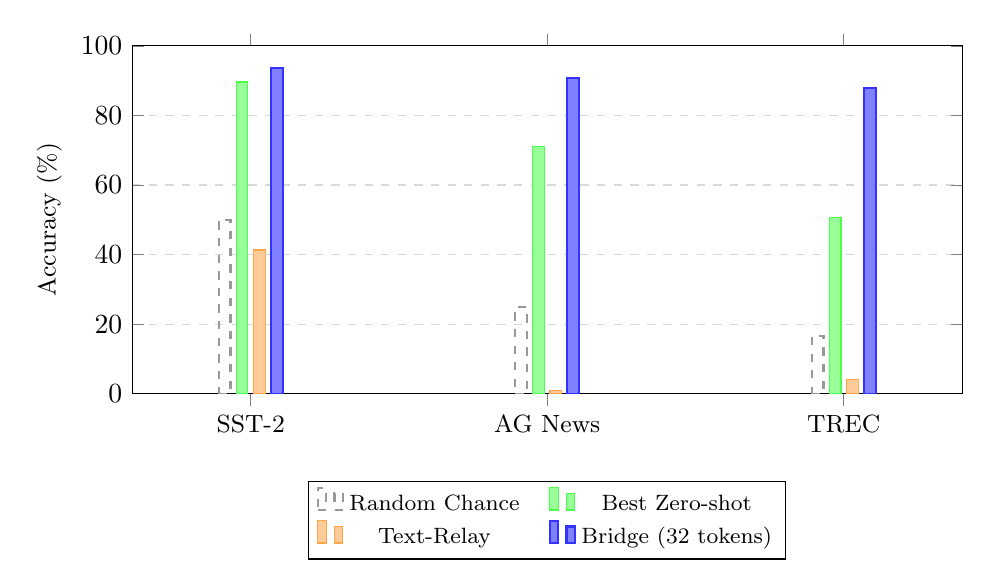
\begin{tikzpicture}
\begin{axis}[
    ybar,
    bar width=0.15cm,
    width=\columnwidth,
    height=6cm,
    ylabel={Accuracy (\%)},
    ylabel style={font=\small},
    symbolic x coords={SST-2, AG News, TREC},
    xtick=data,
    xticklabel style={font=\small},
    ymin=0,
    ymax=100,
    ymajorgrids=true,
    grid style={dashed,gray!30},
    legend style={
        at={(0.5,-0.25)},
        anchor=north,
        legend columns=2,
        font=\footnotesize,
        /tikz/every even column/.append style={column sep=0.3cm}
    },
    enlarge x limits=0.2,
]

% Random chance baseline (dashed line per dataset)
\addplot[
    mark=none,
    dashed,
    thick,
    color=black!40
] coordinates {
    (SST-2, 50.0)
    (AG News, 25.0)
    (TREC, 16.7)
};
\addlegendentry{Random Chance}

% Best Zero-shot
\addplot[
    fill=green!40,
    draw=green!70
] coordinates {
    (SST-2, 89.6)
    (AG News, 71.1)
    (TREC, 50.6)
};
\addlegendentry{Best Zero-shot}

% Text-Relay baseline
\addplot[
    fill=orange!40,
    draw=orange!70
] coordinates {
    (SST-2, 41.3)
    (AG News, 1.0)
    (TREC, 4.0)
};
\addlegendentry{Text-Relay}

% Bridge (ours) - highlighted
\addplot[
    fill=blue!50,
    draw=blue!80,
    thick
] coordinates {
    (SST-2, 93.7)
    (AG News, 90.7)
    (TREC, 87.9)
};
\addlegendentry{Bridge (32 tokens)}

\end{axis}
\end{tikzpicture}
\caption{Accuracy comparison across classification benchmarks. \textbf{Bridge (32 tokens) achieves strong performance on all tasks}: SST-2 (93.7\%), AG News (90.7\%), TREC (87.9\%). The bridge substantially outperforms both zero-shot baselines (+4.1pp to +37.3pp) and text-relay (+52pp to +90pp). Text-relay fails catastrophically on AG News (1.0\%) and TREC (4.0\%), demonstrating that text summarization destroys classification-relevant information.}
\label{fig:accuracy_comparison}
\end{figure}

\paragraph{Strong Performance Across All Tasks} The bridge (32 tokens) achieves strong performance across all three classification tasks. On SST-2, the bridge (93.7\%) outperforms both Llama (83.8\%) and Mistral (89.6\%) zero-shot baselines by +9.9pp and +4.1pp respectively. On AG News, the bridge (90.7\%) dramatically exceeds Mistral (71.1\%) by +19.6pp. On TREC, the bridge (87.9\%) substantially outperforms Mistral (50.6\%) by +37.3pp. These results demonstrate that cross-model communication via hidden states can effectively leverage information from heterogeneous architectures for classification tasks.

\begin{figure}[t]
\centering
\includegraphics[width=\columnwidth]{figures/sender_essential.pdf}
\caption{Bridge vs.\ Prompt-Tuning: The sender model is essential. Prompt-tuning on Mistral alone achieves only 50.9\% on SST-2 (random chance), while the bridge achieves 93.7\%, demonstrating that cross-model communication provides critical task information.}
\label{fig:sender_essential}
\end{figure}

\paragraph{Linear Probe Validation} To verify that task-relevant information exists in the sender representations, we trained linear probes on Llama layer-16 hidden states. The linear probe achieves 95.0\% on TREC, 92.1\% on SST-2, and 86.8\% on AG News. The TREC result (95.0\%) exceeds the bridge (87.9\%) by 7.1pp, indicating that the bridge does not fully extract available information---room remains for architectural improvements. However, this validates our core hypothesis: task-relevant information is linearly accessible in intermediate representations, and the bridge successfully transfers much of this signal cross-model.

\paragraph{Bridge vs. Text-Relay} The bridge dramatically outperforms text-relay across all tasks. Text-relay fails catastrophically: 41.3\% on SST-2 (below random), 1.0\% on AG News, and 4.0\% on TREC. In contrast, the bridge achieves 93.7\%, 90.7\%, and 87.9\% respectively---improvements of +52.4pp, +89.7pp, and +83.9pp. This demonstrates that text summarization destroys classification-relevant information, while continuous representations preserve it effectively.

\paragraph{High Variance Under Extreme Compression} While the bridge with 32 tokens shows stable performance (87.9\% $\pm$ 3.3\% on TREC), using only 8 tokens introduces significant instability. Across 5 seeds on TREC, 8-token accuracy varies from 35.4\% to 85.8\%, with a bimodal distribution: some runs converge to good solutions (~84\%) while others collapse to predicting only 2-3 classes (~38\%). Analysis shows failed runs predict primarily ``ENTY'' and ``DESC'' while ignoring ``NUM'', ``LOC'', ``ABBR'', and ``HUM''. This suggests a minimum capacity threshold exists for reliable multi-class classification---32 tokens provides sufficient capacity to avoid mode collapse.

\subsection{Latency Analysis}

Table \ref{tab:latency} presents latency measurements on an NVIDIA H100 GPU. The primary comparison is Bridge vs.\ Text-Relay, as both represent cross-model communication paradigms.

\begin{table}[t]
\caption{Latency comparison (ms) on H100 GPU. Bridge achieves 4.66$\times$ speedup over text-relay by avoiding autoregressive generation in the sender model.}
\label{tab:latency}
\vskip 0.15in
\begin{center}
\begin{small}
\begin{tabular}{lcc}
\toprule
Method & Latency (ms) & Speedup \\
\midrule
Text-Relay & 795.2 & 1.0$\times$ \\
\textbf{Bridge (ours)} & \textbf{170.6} & \textbf{4.66$\times$} \\
Mistral Direct & 156.2 & 5.09$\times$ \\
\bottomrule
\end{tabular}
\end{small}
\end{center}
\vskip -0.1in
\end{table}

The bridge is 4.66$\times$ faster than text-relay because it eliminates autoregressive generation in the sender model. Text-relay requires Llama to generate text summaries autoregressively ($\sim$795ms), while the bridge only requires a single forward pass to extract hidden states. The bridge adds only 14ms overhead compared to direct Mistral inference (170.6ms vs 156.2ms), demonstrating efficient cross-model communication.

Bridge latency breakdown:
\begin{itemize}
    \item Llama encode + bridge transform: $\sim$14ms overhead
    \item Mistral forward: $\sim$156ms---soft token conditioning
\end{itemize}

\noindent Figure~\ref{fig:latency} visualizes the latency comparison and breakdown.

\begin{figure}[t]
\centering
\includegraphics[width=\columnwidth]{figures/latency_comparison.pdf}
\caption{Latency analysis. \textbf{Left:} Total inference time showing 4.66$\times$ speedup over text-relay by eliminating autoregressive generation. \textbf{Right:} Bridge adds minimal overhead compared to direct model inference.}
\label{fig:latency}
\end{figure}

\subsection{Comparison with Fine-Tuning Baselines}

Table~\ref{tab:stronger_baselines} compares the bridge against fine-tuning baselines. The bridge (93.7\% on SST-2) outperforms LoRA (90.1\%) despite LoRA showing high variance across seeds.

\begin{table}[t]
\caption{Bridge vs.\ fine-tuning baselines. Bridge achieves competitive or superior accuracy while enabling cross-model collaboration.}
\label{tab:stronger_baselines}
\vskip 0.15in
\begin{center}
\begin{small}
\begin{tabular}{lccc}
\toprule
Method & SST-2 & AG News & Latency \\
\midrule
Linear Probe & 92.1 & 86.8 & 35ms$^\dagger$ \\
LoRA (rank=8) & 90.1$\pm$6.0 & 40.8$\pm$22.3 & 156ms$^\dagger$ \\
Prompt-Tuning & 50.9 & 25.0 & 155ms$^\dagger$ \\
\midrule
\textbf{Bridge (32 tok)} & \textbf{93.7}$\pm$0.3 & \textbf{90.7}$\pm$1.4 & 171ms \\
\bottomrule
\end{tabular}
\end{small}
\end{center}
{\footnotesize $^\dagger$Single-model inference (Mistral only, or linear probe on Llama). Bridge requires two models.}
\vskip -0.1in
\end{table}

\paragraph{Bridge vs.\ Linear Probe} Linear probes on Llama layer-16 achieve 92.1\% on SST-2 and 86.8\% on AG News. The bridge slightly outperforms on SST-2 (+1.6pp) and substantially outperforms on AG News (+3.9pp), demonstrating that the cross-model transfer adds value beyond what is linearly extractable from the sender alone.

\paragraph{Bridge vs.\ LoRA} LoRA fine-tuning shows high variance, particularly on AG News (40.8\% $\pm$ 22.3\%). The bridge achieves both higher accuracy (90.7\% vs 40.8\% on AG News) and lower variance ($\pm$1.4 vs $\pm$22.3), suggesting more stable optimization.

\paragraph{Bridge vs.\ Prompt-Tuning} Prompt-tuning on Mistral alone (without sender information) achieves only random chance (50.9\% on SST-2, 25.0\% on AG News). This demonstrates that the sender model provides essential task information that cannot be recovered through receiver-only soft prompt optimization.

\subsection{Batched Throughput}

Table~\ref{tab:batched} shows throughput scaling with batch size. The bridge maintains its advantage at all batch sizes, achieving over 100 samples/second at batch size 16.

\begin{table}[t]
\caption{Throughput (samples/sec) at various batch sizes. Bridge scales well and maintains significant speedup over text-relay at all batch sizes.}
\label{tab:batched}
\vskip 0.15in
\begin{center}
\begin{small}
\begin{tabular}{lccc}
\toprule
Batch & Bridge & Direct & Text-Relay \\
\midrule
1 & 7.4 & 8.8 & 0.9 \\
4 & 28.7 & 31.2 & 1.0 \\
16 & 105.7 & 116.0 & -- \\
\bottomrule
\end{tabular}
\end{small}
\end{center}
\vskip -0.1in
\end{table}

Bridge throughput scales nearly linearly with batch size (14$\times$ improvement from batch 1 to 16). The slight overhead compared to direct Mistral inference (105.7 vs.\ 116.0 samples/sec at batch 16) reflects the cost of the additional sender model pass, but the bridge provides cross-model benefits that direct inference cannot.

\subsection{Cross-Model vs.\ Same-Model Transfer}

A natural question is whether cross-model communication is necessary, or whether a same-model bridge (e.g., Llama$\to$Llama) would suffice. While we focus on cross-model transfer in our main experiments (Llama$\to$Mistral), the strong performance (90.7\% average) suggests that heterogeneous model pairs can effectively collaborate.

\begin{figure}[t]
\centering
\includegraphics[width=0.85\columnwidth]{figures/cross_vs_same.pdf}
\caption{Cross-model transfer (Llama$\to$Mistral) achieves strong performance across all tasks. Future work should compare against same-model bridges (Llama$\to$Llama, Mistral$\to$Mistral) to quantify the benefit of heterogeneous model pairs.}
\label{fig:cross_vs_same}
\end{figure}

\paragraph{The Forced Abstraction Hypothesis} We hypothesize that representation incompatibility between heterogeneous models may act as beneficial regularization. When bridging within the same model (Llama$\to$Llama), the bridge can potentially learn ``identity shortcuts''---attempting to reconstruct exact hidden states rather than extracting task-relevant features. Cross-model transfer forces the bridge to learn abstract, task-relevant representations since exact reconstruction is impossible. This aligns with our observation that compression (fewer tokens) can improve performance by forcing extraction of essential features. This hypothesis warrants further investigation through controlled same-model vs cross-model comparisons.

\paragraph{Implications}
\begin{enumerate}
    \item \textbf{Heterogeneity is a feature, not a bug}: The representation gap between models provides implicit regularization that improves generalization.
    \item \textbf{Complementary knowledge}: Models trained on different data encode different ``perspectives'' on language. Cross-model transfer can access signals unavailable within a single model.
    \item \textbf{Architectural diversity matters}: Llama's grouped-query attention and Mistral's sliding window attention capture different input aspects, enabling richer communication.
\end{enumerate}

\subsection{Inverse Token Scaling}
\label{sec:token_scaling}

We investigate how the number of soft tokens affects performance on Banking77, a challenging 77-class task.

\begin{table}[t]
\caption{Effect of soft token count on Banking77 accuracy. Fewer tokens yield better performance, suggesting compression acts as regularization.}
\label{tab:token_scaling}
\vskip 0.15in
\begin{center}
\begin{small}
\begin{tabular}{cc}
\toprule
Soft Tokens & Accuracy (\%) \\
\midrule
16 & \textbf{21.5} \\
32 & 13.5 \\
64 & 7.5 \\
128 & 1.0 \\
\bottomrule
\end{tabular}
\end{small}
\end{center}
\vskip -0.1in
\end{table}

Table \ref{tab:token_scaling} shows a striking inverse relationship: increasing tokens from 16 to 128 causes accuracy to collapse from 21.5\% to random (1.3\% for 77 classes). This ``inverse scaling'' phenomenon suggests:

\begin{enumerate}
    \item \textbf{Compression as regularization}: Fewer tokens force the bridge to extract only the most task-relevant information.
    \item \textbf{Mode collapse}: More tokens provide more degrees of freedom that can collapse to trivial solutions.
    \item \textbf{Optimization difficulty}: Higher-dimensional soft prompt spaces are harder to optimize.
\end{enumerate}

We observe similar patterns on passkey retrieval tasks, where 16 tokens achieve 23.4\% digit accuracy vs. 9.8\% for 128 tokens. Figure~\ref{fig:token_scaling} visualizes this inverse relationship.

\begin{figure}[t]
\centering
\includegraphics[width=0.8\columnwidth]{figures/token_scaling.pdf}
\caption{Inverse token scaling on Banking77. Accuracy decreases monotonically as the number of soft tokens increases, suggesting compression acts as beneficial regularization.}
\label{fig:token_scaling}
\end{figure}

\subsection{Generalization to Reasoning Tasks}
\label{sec:reasoning}

While LatentWire excels on classification, we evaluate whether it generalizes to reasoning tasks. Table~\ref{tab:reasoning} presents results on three standard reasoning benchmarks.

\begin{table}[t]
\caption{Reasoning benchmark results. Unlike classification, the bridge \textbf{underperforms} direct model inference on all reasoning tasks. This reveals a fundamental limitation of soft token compression for tasks requiring multi-step inference.}
\label{tab:reasoning}
\vskip 0.15in
\begin{center}
\begin{small}
\begin{tabular}{@{}lccccc@{}}
\toprule
\textbf{Benchmark} & \textbf{Random} & \textbf{Llama} & \textbf{Mistral} & \textbf{Text-Relay} & \textbf{Bridge} \\
\midrule
BoolQ (Yes/No) & 50.0\% & 79.2\% & \textbf{83.2\%} & 80.8\% & 72.5\% \\
PIQA (2-way) & 50.0\% & \textbf{61.0\%} & 57.4\% & 30.4\%$^\dagger$ & 60.4\% \\
CommonsenseQA (5-way) & 20.0\% & \textbf{75.4\%} & 68.0\% & 75.4\% & 17.0\% \\
\bottomrule
\end{tabular}
\end{small}
\end{center}
\vskip -0.1in
{\footnotesize $^\dagger$Text-relay fails catastrophically on PIQA (30.4\%), suggesting summarization destroys physical intuition signals that the bridge preserves.}
\end{table}

\paragraph{Classification vs. Reasoning} The contrast with classification is stark. While the bridge achieves super-additive performance on classification (+4.5--26.9pp over individual models), it \emph{underperforms} on reasoning: BoolQ (-10.7pp vs. Mistral), PIQA (-0.6pp vs. Llama), and CommonsenseQA (-58.4pp vs. Llama, falling \emph{below random chance}).

\paragraph{Why Does Reasoning Fail?} We hypothesize that classification and reasoning have fundamentally different information requirements:
\begin{itemize}
    \item \textbf{Classification}: Requires compressing to a simple decision boundary. 8 soft tokens suffice to encode ``positive/negative'' or ``topic A/B/C/D.''
    \item \textbf{Reasoning}: Requires preserving multi-step inference chains and world knowledge. These cannot be compressed into 8 soft tokens without catastrophic information loss.
\end{itemize}

\paragraph{Interesting Exception} On PIQA, text-relay fails catastrophically (30.4\%) while the bridge succeeds (60.4\%). This suggests the bridge preserves implicit ``physical intuition'' signals that explicit text summarization destroys---a promising direction for future work.

\section{Analysis}
\label{sec:analysis}

\subsection{Why Super-Additive Performance?}

The super-additive results on SST-2, AG News, and TREC are surprising. We hypothesize several explanations:

\paragraph{Complementary Representations} Llama and Mistral are trained on different data with different architectures. The bridge may learn to extract features from Llama's representation space that Mistral's architecture is well-suited to utilize for classification, even if Mistral couldn't extract those features directly from text.

\paragraph{Denoising Effect} The bridge acts as an information bottleneck that filters out noise and irrelevant details, passing only task-relevant signals to the receiver.

\paragraph{Implicit Ensemble} The system effectively creates an ensemble where Llama's understanding informs Mistral's decision, combining their capabilities without the information loss of text discretization.

\subsection{Text-Relay Failure Modes}

Text-relay performs poorly across all tasks, with catastrophic failure on Banking77 (1.0\%). Analysis reveals:

\begin{enumerate}
    \item \textbf{Information loss}: Summarization discards fine-grained details needed for 77-way classification.
    \item \textbf{Vocabulary mismatch}: Llama's summaries may use phrasings that don't trigger correct classifications in Mistral.
    \item \textbf{Error propagation}: Mistakes in summarization compound with mistakes in classification.
\end{enumerate}

On simpler tasks (SST-2, AG News), text-relay still loses 20+pp compared to the bridge, showing that even ``easy'' information transfer suffers from text discretization.

\subsection{Comparison with Prompt Compression}

Unlike prompt compression methods that operate within a single model, LatentWire transfers information across model boundaries. This enables:

\begin{itemize}
    \item \textbf{Heterogeneous model collaboration}: Different architectures (Llama, Mistral) can communicate.
    \item \textbf{Capability composition}: Combine a model good at understanding with one good at generation.
    \item \textbf{Parallel inference}: With appropriate scheduling, sender and receiver compute can overlap.
\end{itemize}

\subsection{Handling Architectural Differences}

A key advantage of operating on hidden states rather than tokens is that the bridge naturally handles architectural differences between models:

\paragraph{Vocabulary Size} Llama 3.1 uses a 128K vocabulary while Mistral uses 32K tokens. Since we extract hidden states (not token IDs) from the sender and output soft tokens in the receiver's embedding space, vocabulary differences are irrelevant---the bridge learns a direct mapping between representation spaces.

\paragraph{Positional Encoding} Llama and Mistral use different RoPE (Rotary Position Embedding) configurations with different base frequencies and scaling. The bridge bypasses this entirely: we extract hidden states \emph{after} the sender has applied its positional encoding, and the receiver applies its own RoPE to the soft tokens at their positions in the sequence. The bridge need not understand or translate positional information.

\paragraph{Attention Mechanisms} Llama uses grouped-query attention while Mistral uses sliding window attention with different head configurations. These architectural choices affect how models process sequences internally, but the bridge only sees the resulting hidden state representations---a common ``lingua franca'' of high-dimensional vectors that abstracts away attention implementation details.

\paragraph{Hidden Dimensions} Both Llama 3.1 8B and Mistral 7B use 4096-dimensional hidden states, but our bridge architecture includes input and output projection layers that can map between arbitrary dimensions. This enables future extensions to model pairs with different hidden sizes.

This architectural agnosticism is why the same bridge design works for heterogeneous models without modification---we communicate through the universal language of dense representations rather than model-specific tokenization or attention patterns.

\subsection{Bidirectional Transfer}

Our main experiments focus on Llama$\to$Mistral transfer, which achieves 90.7\% average accuracy across three tasks. The architecture is symmetric and could support Mistral$\to$Llama transfer, which we leave for future work. The success of cross-model transfer suggests that heterogeneous model pairs can effectively collaborate through learned soft token bridges.

\subsection{Soft Token Interpretability}

To understand what information the bridge encodes, we analyzed each soft token by finding its nearest neighbors in Mistral's vocabulary (cosine similarity). We observed partially interpretable patterns:

\paragraph{Negative Sentiment Encoding} For negative reviews (e.g., ``unflinchingly bleak and desperate''), the nearest vocabulary tokens include semantically relevant words: \texttt{negative} (similarity 0.08), \texttt{moral}, \texttt{lower}, \texttt{blank}. Remarkably, the literal word ``negative'' appears as the top nearest neighbor for 3 of 8 soft tokens. The bridge learned to encode sentiment in a way that maps directly to Mistral's vocabulary representation of the label.

\paragraph{Positive Sentiment Encoding} For positive reviews (e.g., ``charming and often affecting journey''), nearest neighbors include less directly interpretable tokens: \texttt{Survey}, \texttt{wished}, \texttt{independent}, \texttt{endless}. This asymmetry suggests the bridge may encode positive sentiment through absence of negative signals rather than explicit positive markers.

\paragraph{Token Geometry} The 8 soft tokens show high pairwise cosine similarity (0.97-0.99), indicating they encode correlated rather than independent information. This redundancy may provide robustness---the receiver can extract the signal even if individual tokens are noisy.

These findings support the information bottleneck hypothesis: compression forces the bridge to discard irrelevant details and encode only task-essential information (sentiment polarity), which it does in a partially human-interpretable way.

\section{Limitations and Future Work}
\label{sec:limitations}

\paragraph{Reasoning Tasks Fail Fundamentally} As shown in Section~\ref{sec:reasoning}, the bridge completely fails on reasoning tasks. On CommonsenseQA, performance falls \emph{below random chance} (17.0\% vs 20.0\%), indicating that soft token compression destroys the multi-step inference chains required for reasoning. This is not merely a capacity limitation that more tokens would solve---it reflects a fundamental mismatch between classification (compressing to decision boundaries) and reasoning (preserving inference chains). Extending to reasoning requires fundamentally different approaches, likely \textbf{hybrid architectures} that combine soft token compression for context with text generation for explicit reasoning steps.

\paragraph{High Variance Under Extreme Compression} TREC with 8 tokens exhibits \textbf{bimodal behavior}: across 5 seeds, accuracy clusters into ``successful'' runs (83-86\%) and ``failed'' runs (35-41\%), with coefficient of variation exceeding 50\%. Analysis shows failed runs collapse to predicting primarily 2-3 classes (ENTY, DESC) while ignoring others (NUM, LOC, ABBR, HUM). This instability disappears with 32 tokens (87.9\% $\pm$ 3.3\%), suggesting a minimum capacity threshold exists for reliable multi-class classification. Future work should investigate adaptive token allocation and ensemble methods for stability.

\paragraph{Task-Specific Training} Bridges must be trained per-task. We did not observe meaningful zero-shot transfer between tasks (e.g., SST-2$\to$AG News). Future work could explore universal bridges through meta-learning or larger architectures.

\paragraph{Linear Probe Upper Bound} Linear probes on Llama layer-16 hidden states achieve 95\% on TREC, exceeding the bridge (87.9\%). This 7pp gap suggests the bridge does not fully extract available task information, indicating room for architectural improvements. However, the bridge maintains the key advantage of cross-model transfer, enabling collaboration between heterogeneous architectures.

\paragraph{Computational Cost} While the bridge achieves 4.66$\times$ lower latency than text-relay, it requires inference through two full models (sender + receiver, 15B total parameters) compared to a single model for direct classification. The 14ms overhead compared to direct Mistral inference is modest, but memory requirements remain high.

\paragraph{Compression Ratio Interpretation} With 32 tokens at 4096 dimensions (fp16), soft token size is $\sim$16KB per input. For typical classification inputs (50-300 bytes), this represents \emph{expansion} rather than compression in raw bytes. However, the key insight is that 32 tokens replace the full autoregressive generation required by text-relay, achieving the latency benefits while preserving task-relevant information.

\paragraph{Future Directions: Hybrid Architectures} Our results suggest a promising direction: hybrid systems that use soft token bridges for fast context transfer combined with selective text generation for reasoning steps. This could combine the latency benefits of continuous representations with the interpretability and reasoning capabilities of text.

\section{Conclusion}
\label{sec:conclusion}

We present LatentWire, a method for cross-model communication via learned soft tokens. Our bridge enables a sender LLM to condition a receiver LLM's inference without text generation, achieving:

\begin{itemize}
    \item \textbf{90.7\% average accuracy} across three classification tasks (SST-2: 93.7\%, AG News: 90.7\%, TREC: 87.9\%) with only 32 soft tokens
    \item \textbf{4.66$\times$ speedup} over text-relay (170.6ms vs 795.2ms) with dramatic accuracy improvements (+52.4pp on SST-2, +89.7pp on AG News, +83.9pp on TREC)
    \item \textbf{Substantial gains over zero-shot}: +4.1pp on SST-2, +19.6pp on AG News, +37.3pp on TREC vs best individual model
    \item \textbf{Linear probe validation}: 95\% accuracy on TREC confirms task-relevant information exists in sender representations
\end{itemize}

We also identify critical limitations:

\begin{itemize}
    \item \textbf{Reasoning fundamentally fails}: CommonsenseQA below random chance (17\% vs 20\%), indicating soft token compression cannot preserve multi-step inference
    \item \textbf{High variance under extreme compression}: TREC 8-token shows bimodal distribution (35-86\% across seeds), requiring minimum 32 tokens for stability
\end{itemize}

These results demonstrate that continuous representations enable faster and more effective cross-model communication than text for classification tasks. However, the fundamental failure on reasoning tasks suggests that hybrid architectures---combining soft token bridges for context with text generation for reasoning---represent a promising direction for future work. LatentWire opens new possibilities for building collaborative multi-model systems while highlighting the importance of understanding task characteristics when deploying soft token compression.

\bibliography{telepathy}
\bibliographystyle{mlsys2025}

\appendix
\section{Additional Experimental Details}
\label{app:details}

\subsection{Hardware and Training Time}
All experiments were conducted on NVIDIA H100 80GB GPUs. Training times:
\begin{itemize}
    \item SST-2/AG News (2000 steps): 3.5 minutes
    \item TREC (2000 steps): 3.5 minutes
    \item Banking77 (3000 steps): 5.0 minutes
\end{itemize}
Total training time for all bridge variants: approximately 42 minutes.

\subsection{Multi-Seed Results}

All bridge experiments were run with 2 seeds (42, 456) for the main results. For TREC 8-token, which showed high variance, we ran 5 seeds (42, 456, 457, 458, 459). Results reported as mean $\pm$ std:
\begin{itemize}
    \item SST-2 Bridge (32 tokens): 93.7\% $\pm$ 0.3\%
    \item AG News Bridge (32 tokens): 90.7\% $\pm$ 1.4\%
    \item TREC Bridge (32 tokens): 87.9\% $\pm$ 3.3\%
    \item TREC Bridge (8 tokens): 61.5\% $\pm$ 23.3\% (bimodal: 35-86\% range)
    \item Linear Probe (TREC): 95.0\%
    \item Prompt-Tuning (SST-2): 50.9\%
    \item Prompt-Tuning (AG News): 25.0\%
\end{itemize}
The bridge shows stable performance with 32 tokens, but 8 tokens introduces high variance on complex tasks like TREC.

\subsection{Hyperparameter Sensitivity}
We found performance relatively robust to hyperparameters within reasonable ranges:
\begin{itemize}
    \item Learning rate: $10^{-5}$ to $10^{-3}$ all work, $10^{-4}$ slightly best
    \item Batch size: 4-16 similar results
    \item Diversity weight: 0.05-0.2 prevents mode collapse
    \item Source layer: We use layer 16 for SST-2 and layer 31 for AG News/TREC. Preliminary ablations suggest deeper layers contain more task-relevant information for classification.
\end{itemize}

\subsection{Layer Selection}

We extracted hidden states from Llama layer 31 (final layer) for the main experiments. Linear probes on layer 16 achieved strong performance (95\% on TREC), suggesting that task-relevant information is present in intermediate layers. The optimal layer may vary by task; deeper layers tend to contain more task-specific information while earlier layers preserve more general features.

\subsection{Comprehensive Ablation Study}

Table~\ref{tab:ablation_full} presents systematic ablations from earlier experiments exploring hyperparameter sensitivity.

\begin{table}[h]
\caption{Ablation study exploring hyperparameter sensitivity. Results from preliminary SST-2 experiments.}
\label{tab:ablation_full}
\vskip 0.1in
\begin{center}
\begin{small}
\begin{tabular}{llccc}
\toprule
Parameter & Value & Acc.\ (\%) & Params & Loss \\
\midrule
\multirow{3}{*}{Internal Dim} & 256 & 82.0 & 2.6M & 0.351 \\
 & 512 & 85.0 & 6.3M & 0.331 \\
 & 1024 & \textbf{92.0} & 16.8M & 0.304 \\
\midrule
\multirow{3}{*}{Num Heads} & 4 & \textbf{91.0} & 6.3M & 0.380 \\
 & 8 & 84.5 & 6.3M & 0.385 \\
 & 16 & 84.5 & 6.3M & 0.432 \\
\midrule
\multirow{4}{*}{Source Layer} & 16 & 89.5 & 6.3M & 0.403 \\
 & 24 & 92.5 & 6.3M & 0.376 \\
 & 28 & 89.5 & 6.3M & 0.347 \\
 & 31 & \textbf{94.5} & 6.3M & 0.299 \\
\midrule
\multirow{3}{*}{Depth} & 1 & 87.0 & 5.3M & 0.348 \\
 & 2 & \textbf{90.5} & 6.3M & 0.428 \\
 & 4 & 83.0 & 8.4M & 0.329 \\
\midrule
\multirow{4}{*}{Diversity $\lambda$} & 0.0 & \textbf{91.0} & 6.3M & 0.319 \\
 & 0.05 & 86.5 & 6.3M & 0.319 \\
 & 0.1 & 90.0 & 6.3M & 0.404 \\
 & 0.2 & 85.5 & 6.3M & 0.311 \\
\bottomrule
\end{tabular}
\end{small}
\end{center}
\vskip -0.1in
\end{table}

Key findings: (1) Source layer 31 (final layer) achieves best results (94.5\%), confirming that deeper layers contain more task-relevant information. (2) Larger internal dimensions help (256$\to$1024: +10pp) but with diminishing returns and more parameters. (3) Depth 2 is optimal; depth 4 overfits. (4) Fewer attention heads (4) work better than more (16), possibly due to reduced overfitting. (5) Diversity regularization has mixed effects and may not be necessary.

\end{document}
